\section{Transformer} \label{sec:Transformer}

\begin{figure}[h]
\vspace{-10pt}
\centering
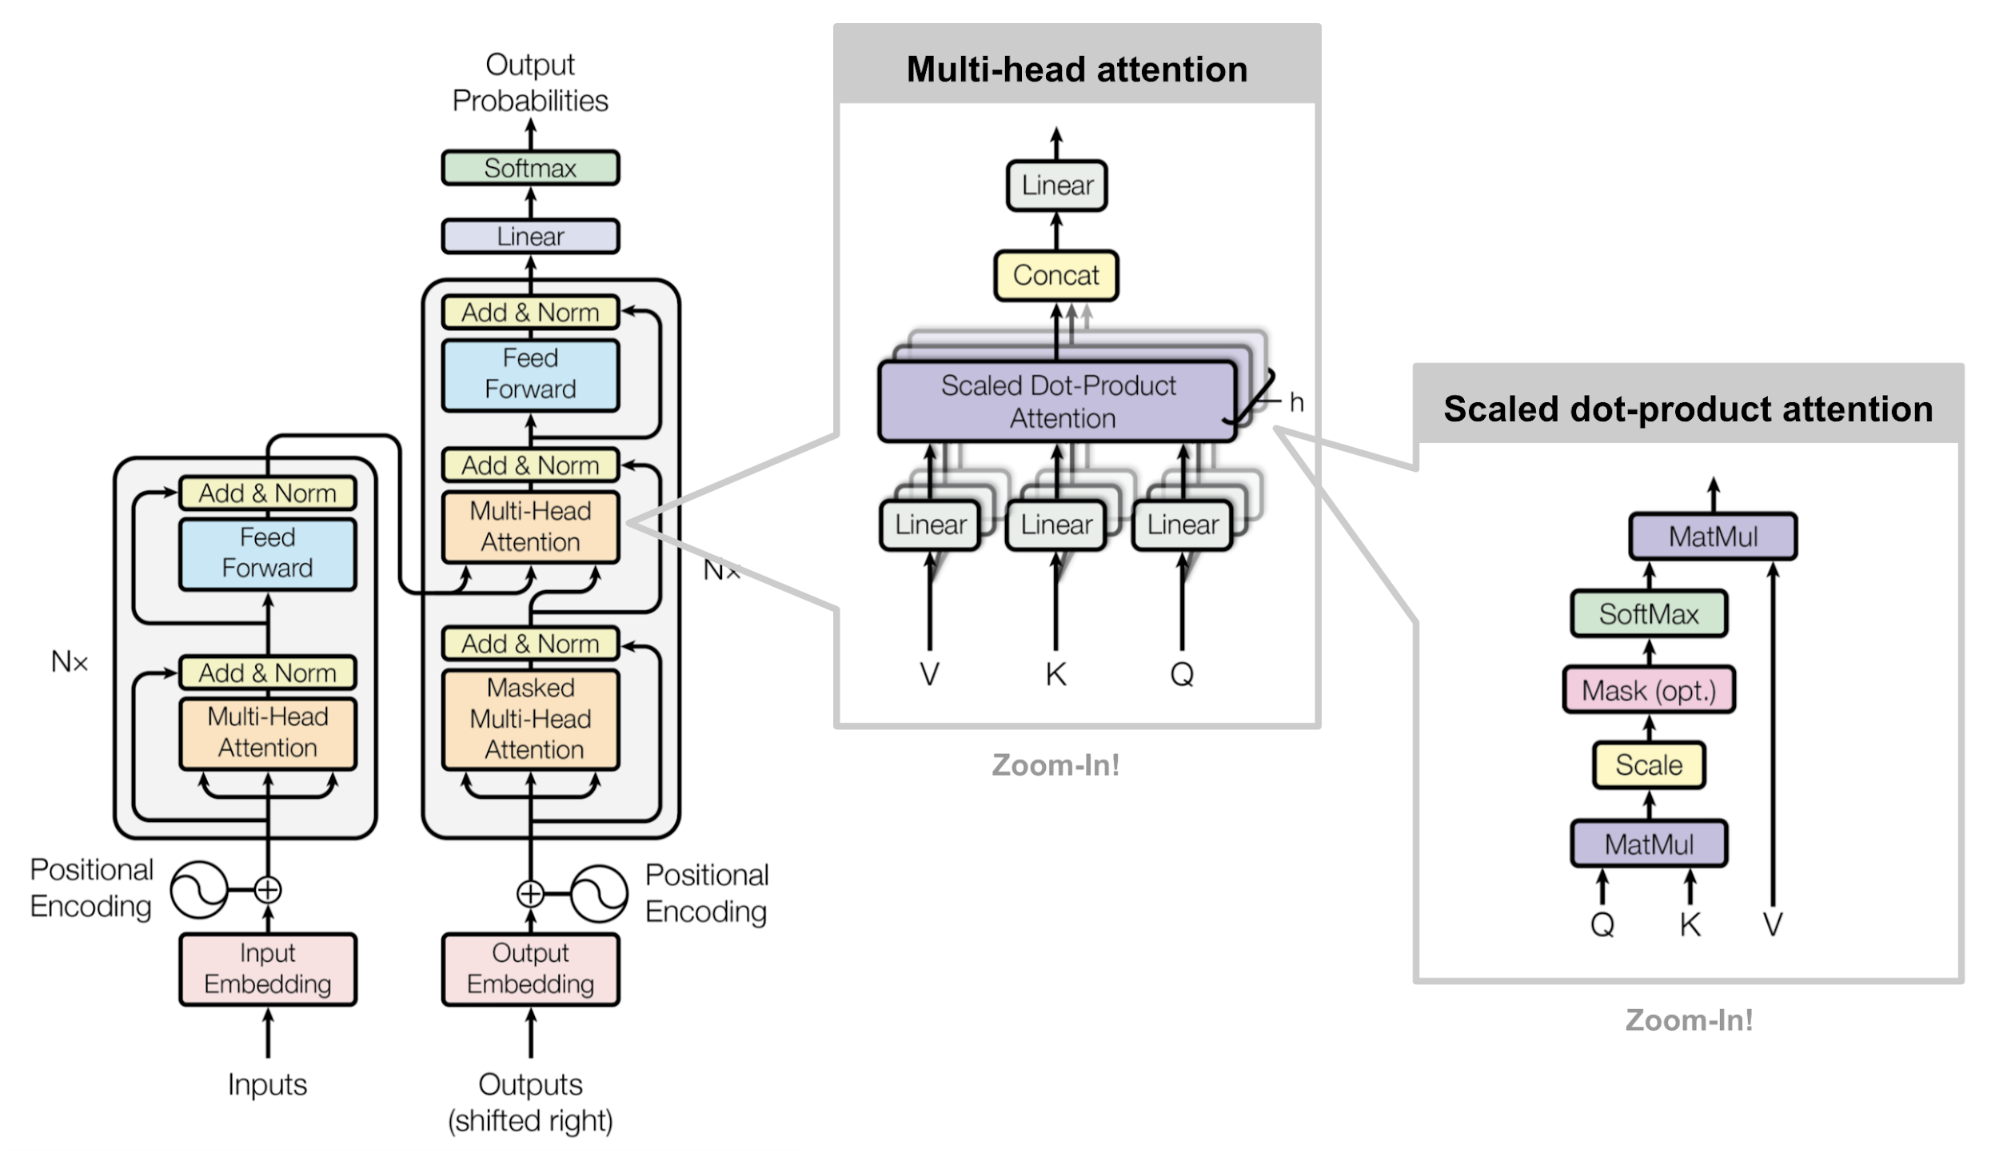
\includegraphics[width=0.95\textwidth]{imgs/transformer.png}
\vspace{-10pt}
\caption{\footnotesize Transformer model architecture. The gray boxes hold Encoder and Decoder layers, respectively, which are each repeated $N=6$ times. From \emph{Attention? Attention}, by Weng, 2018. \url{https://lilianweng.github.io/lil-log/2018/06/24/attention-attention.html}. Copyright 2018 by Weng.}
\vspace{-5pt}
\label{fig:transformer}
\end{figure}

The \textbf{Transformer model} introduced by Vaswani et al. (2017) for \nameref{nlptask:neuralmachinetranslationNMT} proves more parallelizable than general seq-to-seq models with attention. Rather than using \hyperref[sec:RNN]{ recurrent neural networks (RNNs)} combined with the \textbf{\hyperref[sec:AttentionMechanism]{attention mechanism}}, the Transformer sequence-to-sequence model uses only a \textbf{\hyperref[sec:SelfAttention]{self attention mechanism}} to attend to different word tokens in an input sentence and thus generate a sequence of \hyperref[sec:SolutionWithContextEmbs]{contextual embeddings}. It is illustrated in \cref{fig:transformer}.




\subsection{Self-Attention} \label{sec:SelfAttention}

\subsubsection{Motivation for Self-Attention}

{\large \textit{``The animal didn't cross the road because it was too tired."}}

%\begin{shadequote}{}
%\vspace{10pt}
%\large \textit{The animal didn't cross the road because it %was too tired.}
%\vspace{10pt}
%\end{shadequote}

What does ``it” in this sentence refer to? Is ``it" referring to the road or to the animal? This question may be simple to a human but not to a machine.  

This is the motivation for \textbf{self-attention}: when the Transformer processes the word ``it", self-attention allows it to associate ``it" with ``animal". As the Transformer processes each word, self-attention allows it to look at other positions in the input sentence for clues to create a better encoding for this word. In each layer, a part of the attention mechanism that focuses on ``the animal" was \emph{baked in} to a part of the representation of the word ``it" when encoding this in the model (Trevett, 2020). 


\subsubsection{Query, Key, Value} \label{sec:QKV}

Formally, ``an \textbf{\textit{attention function}} can be described as mapping a query and a set of key-value pairs to an output, where the \textbf{query, keys, values}, and output are all vectors. The output is computed as a weighted sum of the values, where the weight assigned to each value is computed by a compatibility function of the query with the corresponding key" (Vaswani et al., 2017). 

\begin{itemize}
    \item The Query matrix $Q$ contains row-wise information for which word to calculate self attention. 
    
     \item The Key matrix $K$ holds word vector representations on its rows, for \emph{each} word in the sentence.
     
    \item The Value matrix $V$ contains vector row-wise information for the rest of the words in the sentence. Multiplying the query vector with the key vector of a particular word, stored in $Q$ and $K$ computes a result that indicates how much \emph{value} vector $V$ to consider.
\end{itemize}

For the previous sentence, ``The animal didn't cross the road because it was too tired,"  $Q$ query refers to the word ``it"; $V$ contains vectors for words other than ``it", and $K$ contains vectors for each word, including ``it".  

The final embedding of the word or \textbf{output} is a weighted sum of \textbf{value} vectors and \hyperref[cnc:softmaxLayer]{softmax probabilities} of the dot product between query and key vectors: 
$$
Attention \Big(Q, K, V \Big) = softmax \Bigg(\frac {QK^T} {\sqrt{d_k}} \Bigg) V
$$
Each word has an associated \textbf{query, key, value} vector which are created by multiplying the words embeddings with parameter weight matrices $W^Q, W^K, W^V$ that are associated with the query, key, and value matrices, respectively. For the example sentence, let the input be the matrix $X = \{\overrightarrow{x_1}, \overrightarrow{x_2}, ..., \overrightarrow{x_n}\}$, where vector $\overrightarrow{x_i}$ corresponds to word $\overrightarrow{w_i}$, and there are $n$ words. Then the input word vectors are: 
% $
% \overrightarrow{x_1} = \text{"The"}, \!
% \overrightarrow{x_2} = \text{"animal"}, \!
% \overrightarrow{x_3} = \text{"didn't"}, \!
% \overrightarrow{x_4} = \text{"cross"}, \!
% \overrightarrow{x_5} = \text{"the"}, \!
% \overrightarrow{x_6} = \text{"road"}, \!
% \overrightarrow{x_7} = \text{because"}, \!
% \overrightarrow{x_8} = \text{"it"}, \!
% \overrightarrow{x_9} = \text{"was"}, \!
% \overrightarrow{x_{10}} = \text{"too"}, \!
% \overrightarrow{x_{11}} = \text{"tired"}, \!
% \overrightarrow{x_{12}} = "." 
% $

$$
\begin{array}{ll}
\overrightarrow{x_1} = \text{"The"} \\
\overrightarrow{x_2} = \text{"animal"} \\
\overrightarrow{x_3} = \text{"didn't"} \\
\overrightarrow{x_4} = \text{"cross"} \\
\overrightarrow{x_5} = \text{"the"} \\
\overrightarrow{x_6} = \text{"road"} \\
\overrightarrow{x_7} = \text{because"} \\
\overrightarrow{x_8} = \text{"it"} \\
\overrightarrow{x_9} = \text{"was"} \\
\overrightarrow{x_{10}} = \text{"too"} \\
\overrightarrow{x_{11}} = \text{"tired"} \\
\overrightarrow{x_{12}} = "." \\
\end{array}
$$
and the corresponding word embedding vectors are denoted $\Big\{ \overrightarrow{w_1}, \overrightarrow{w_2}, ..., \overrightarrow{w_n} \Big\}$ and the \textbf{query, key, value} matrices are denoted $Q = \Big\{\overrightarrow{q_1}, \overrightarrow{q_2}, ..., \overrightarrow{q_n} \Big\}$, $K = \Big\{\overrightarrow{k_1}, \overrightarrow{k_2}, ..., \overrightarrow{k_n} \Big\}$, $V = \Big\{\overrightarrow{v_1}, \overrightarrow{v_2}, ..., \overrightarrow{v_n} \Big\}$ respectively.


\subsubsection{Self-Attention: Vector Calculation}

Using notation from Vaswani et al. (2017) and Alammar (2018b), 

\begin{enumerate}
    \item \textbf{Create Query, Key, Value Vectors}: The first step is to create query, key, value vectors from each of the Encoder's input word embeddings $\overrightarrow{w_i}$ corresponding each word $\overrightarrow{x_i}$ by multiplying the embedding by appropriate rows in the three matrices obtained during training.  

    \item \textbf{Calculate a Score}: The scores determine how much \emph{focus to place on other parts of the input sentence} while encoding a word at a certain position.  The score is calculated by taking the dot product of the \textbf{query} vector with the \textbf{key} vector of the respective word being scored. Thus for word $\overrightarrow{w_i}$, the scores are: 
    $$
    \text{scores}_{\Large w_i} = \bigg\{
    \overrightarrow{q_i} \cdot \overrightarrow{k_1},
    \overrightarrow{q_i} \cdot \overrightarrow{k_2},
    ...,
    \overrightarrow{q_i} \cdot \overrightarrow{k_n} \bigg\}
    $$

    \item \textbf{Scale The Score}: The scores are scaled using $d_k$, which is the dimension of the key vector. From Vaswani et al. (2017), ``for large values of $d_k$, the dot products grow large in  magnitude, forcing the \hyperref[cnc:softmaxLayer]{softmax function} into regions where it has extremely small gradients. To counteract this effect, we scale the dot products by $\frac {1} {\sqrt{d_k}}$." Thus the scores for $\overrightarrow{w_i}$ are:
    $$
    \text{scores}_{\overrightarrow{w_i}} = \Bigg\{
    \frac {\overrightarrow{q_i} \cdot \overrightarrow{k_1}} {\sqrt{d_k}},
    \frac {\overrightarrow{q_i} \cdot \overrightarrow{k_2}} {\sqrt{d_k}},
    ...,
    \frac{\overrightarrow{q_i} \cdot \overrightarrow{k_n}} {\sqrt{d_k}} \Bigg\}
    $$
    
    \item \textbf{Apply Softmax}: The \hyperref[cnc:softmaxLayer]{softmax function} normalizes the scores into probabilities. 
    $$
    \text{scores}_{\overrightarrow{w_i}} = softmax \Bigg( \Bigg\{
    \frac {\overrightarrow{q_i} \cdot \overrightarrow{k_1}} {\sqrt{d_k}},
    \frac {\overrightarrow{q_i} \cdot \overrightarrow{k_2}} {\sqrt{d_k}},
    ...,
    \frac{\overrightarrow{q_i} \cdot \overrightarrow{k_n}} {\sqrt{d_k}} \Bigg\} \Bigg)
    $$

    \item \textbf{Compute the Weights}: The weighted values for word embedding $\overrightarrow{w_i}$ are calculated by multiplying each value vector in matrix $V$ by the \hyperref[cnc:softmaxLayer]{softmax} scores. Intuitively, this cements the values of words to focus on while drowning out irrelevant words. 
    $$
    \text{weights}_{\overrightarrow{w_i}} = \text{scores}_{\overrightarrow{w_i}} * (\overrightarrow{v_1}, ..., \overrightarrow{v_n})
    $$

    \item \textbf{Compute Output Vector}: The weight vector's cells are summed to produce the \textbf{output vector} of the self-attention layer for word embedding $\overrightarrow{w_i}$: 
    $$
    \overrightarrow{output_{w_i}} = softmax \Bigg(
    \frac {\overrightarrow{q_i} \cdot \overrightarrow{k_1}} {\sqrt{d_k}} \Bigg) \cdot \overrightarrow{v_1} +
    softmax \Bigg(\frac {\overrightarrow{q_i} \cdot \overrightarrow{k_1}} {\sqrt{d_k}} \Bigg) \cdot \overrightarrow{v_2} + ... +
    softmax \Bigg(\frac {\overrightarrow{q_i} \cdot \overrightarrow{k_1}} {\sqrt{d_k}} \Bigg) \cdot \overrightarrow{v_n}
    $$
\end{enumerate} 


\subsection{Self-Attention: Matrix Calculation}

Using notation from Vaswani et al. (2017) and Alammar (2018b), 

\begin{enumerate}
    \item \textbf{Calculate Query, Key, Value Matrices}: The word embeddings are packed into the rows of input matrix $X$ and this is multiplied by each of the trained parameter matrices $W^Q$, $W^K$, $W^V$ to produce the $Q$, $K$, $V$ matrices:
    $$
    \begin{array}{ll}
    Q = X \cdot W^Q \\
    K = X \cdot W^K \\
    V = X \cdot W^V 
    \end{array}
    $$
    
    \item \textbf{Calculate Self Attention}: Steps 2 through 6 of the vector calculation for self attention can be condensed into a single matrix step where $Q = \Big\{\overrightarrow{q_1}, \overrightarrow{q_2}, ..., \overrightarrow{q_n} \Big\}$, $K = \Big\{\overrightarrow{k_1}, \overrightarrow{k_2}, ..., \overrightarrow{k_n} \Big\}$, $V = \Big\{\overrightarrow{v_1}, \overrightarrow{v_2}, ..., \overrightarrow{v_n} \Big\}$: 
    $$
    Attention(Q, K, V) = softmax \Bigg(\frac {QK^T} {\sqrt{d_k}} \Bigg) \cdot V
    $$
\end{enumerate}


\subsection{Multi-Head Attention} \label{sec:MultiHeadAttention}

\subsubsection{Motivation for Multi-Head Attention}


A \textbf{multi-head attention mechanism} comprises of several self-attention heads, enabling the Transformer to ``jointly attend to information from different representation subspaces at different positions." A single attention head cannot do this because of averaging (Vaswani et al., 2017).  

While a single attention function has $d_{model}$-dimensional keys, values and queries, a multi-head attention function ``linearly projects the queries, keys and values $H$ (number of attention heads) times with different, learned linear projections to $d_k$, $d_k$, and $d_v$ dimensions, respectively." Instead of calculating attention once, multi-head attention does self attention many times in parallel on the projected dimensions, concatenates the independent attention outputs, and once again projects the result into the expected dimension to give a final value (Vaswani et al., 2017; Weng, 2018).  

For the example sentence, adding more attention heads enables the Transformer to focus on different words while encoding the meaning of word ``it." As ``it" is encoded, one attention head may focus most on ``the animal" while another focuses on ``tired", so the model's representation of ``it" incorporates some representation of all the words in the sentence (Trevett, 2020). 

\subsubsection{Multi-Head Attention: Matrix Calculation}

Using notation from Vaswani et al. (2017) and Alammar (2018b): 

\begin{enumerate}
    \item \textbf{Create $Q$, $K$, $V$ matrices}: With multi-headed attention there are now separate $Q$, $K$, $V$ weight matrices for each attention head $h$, in $1 \leq h \leq H$. The rows of input matrix $X$ correspond to a word in the input sentence, as before. For each attention head, $X$ is multiplied by trained parameter matrices to produce the separate query, key, value matrices: 
    $$
    Q_h = X \cdot W_h^Q \\
    K_h = X \cdot W_h^K \\
    V_h = X \cdot W_h^V 
    $$
    where $H =$ number of attention heads, and the dimensions of the parameter matrices are $\large W_h^Q \in \mathbb{R}^{\Large d_{model} \times d_k}$, $\large W_h^K \in \mathbb{R}^{\Large d_{model} \times d_k}$, $\large W_h^V \in \mathbb{R}^{\Large d_{model} \times d_v}$. 
    
    \item \textbf{Apply Softmax To Get Output Matrix}: Steps two through six in the vector calculation of self-attention can be condensed in a single matrix step to find the final output matrix $Z_h$ for the $h$-th attention head for any self-attention layer:
    $$
    Z_h := softmax \Bigg(\frac {Q_h K_h^T} {\sqrt{d_k}} \Bigg) \cdot V_h
    $$
    
    \item \textbf{Concatenate Output Matrices}: Now there are $H$ different output matrices $Z$ for each attention head. But the feed-forward layer is only expecting a single matrix instead of $H$. Thus, this step concatenates the $H$ matrices and multiplies the result by an additional weights matrix $W^O$ to return to expected dimensions. 
    $$
    MultiHeadAttention(Q, K, V) = Concat(head_1, ..., head_H) \cdot W^O
    $$
      where $head_i = Attention(Q \cdot W_h^Q, K \cdot W_h^K, V \cdot W_h^V)$, where the attention function is simply $Attention(Q, K, V) = softmax \Bigg( \frac {\Large QK^T} {\Large \sqrt{d_k}} \Bigg) \cdot V$. The parameter matrices have the following dimensions:  $W^O \in \mathbb{R}^{\Large H \cdot d_v \times d_{model}}$, $\large W_h^Q \in \mathbb{R}^{\Large d_{model} \times d_k}$, $\large W_h^K \in \mathbb{R}^{\Large d_{model} \times d_k}$, $\large W_h^V \in \mathbb{R}^{\Large d_{model} \times d_v}$
    
    
\end{enumerate}



\subsection{Positional Encodings} \label{sec:PosEncodings}

\subsubsection{Motivation for Positional Encodings}

Since the Transformer contains no recurrence mechanism it does not yet account for \emph{order in the sequence sentence}. Vaswani et al. (2017) found that injecting information about relative or absolute position of tokens in the sequence in the form of \textbf{positional encodings} helps resolve this issue. 
Otherwise, the sentences ``I like dogs more than cats" and ``I like cats more than dogs" would encode the same meaning (Raviraja, 2019). 

\subsubsection{Describing Positional Encodings}

A \textbf{positional encoding} follows a specific, learned pattern to identify word position or the distance between words in the sequence (Alammar, 2018b). The Transformer adds the positional encoding vector to each input embedding in both Encoder and Decoder stacks.   

According to Vaswani et al. (2017), positional encodings use sinusoidal waves to allow the Transformer to more easily attend to relative positions since for any fixed offset $k$, the positional encoding $\textit{PosEnc}_{\textit{pos} + k}$ can be represented as a linear function of $\textit{PosEnc}_{\textit{pos}}$.
$$
\begin{array}{ll}
\textit{PosEnc}_{\Large (\textit{pos}, 2i)} = \text{sin} \Bigg(\frac {\textit{pos}} {10000^{\Large \frac {2i} {d_{\textit{model}}} } }  \Bigg) \\
\textit{PosEnc}_{\Large (\textit{pos}, 2i + 1)} = \text{cos} \Bigg(\frac {\textit{pos}} {10000^{\Large \frac {2i} {d_{\textit{model}}} } }  \Bigg)
\end{array}
$$
where $\textit{pos} = $ a position, $i = $ a dimension.


\subsection{Position-wise Feed Forward Layer} \label{sec:PositionwiseFFNLayers}

A \textbf{positionwise feed-forward layer} is a kind of \hyperref[sec:NeuralNetRepr]{feed-forward neural network (FNN)} that is also ``position-wise" because the FFN is applied to each position separately and identically. The FFN contains two linear transformations with a $\textit{ReLU}$ or $\textit{max}$ activation function in between them:
$$
\textit{FFN}(x) = \textit{ReLU}(0, x W_1 + b_1) W_2 + b_2
$$

\subsection{Residual Connection} \label{sec:ResidualConnections}

A \textbf{residual connection} is a sub-layer in both Encoder and Decoder stacks which adds inputs to outputs of a sub-layer. This allows gradients during optimization to flow through a network directly rather than being transformed by nonlinear activations (Raviraja, 2019): 
$$
\textit{LayerNorm}(x + \textit{Sublayer}(x))
$$
where $\textit{Sublayer}(x)$ is a general function representing the sub-layer's operation. Each sub-layer in the stack, such as \hyperref[sec:SelfAttention]{self-attention} and \hyperref[sec:PositionwiseFFNLayers]{positionwise feed forward layer}s, are surrounded by residual connection layers followed by layer normalization. 




\subsection{Masked Multi-Head Attention} \label{sec:MaskedMultiHeadAttention}

The \textbf{masked self attention} is an \hyperref[sec:AttentionMechanism]{attention mechanism} that forms a sub-layer in the Decoder stack. It uses \textbf{masking} to prevent positions from attending to subsequent positions. Rather, while decoding a word embedding $\overrightarrow{w_i}$, the Decoder is not aware of words  $\overrightarrow{w_{>i}}$ past position $i$. It can only use words $\overrightarrow{w_{\leq i}}$. This masking is done to render invisible the words $\overrightarrow{w_{>i}}$ so that no superfluous predictions can be made (Ta-Chun, 2018). 

\subsection{Encoder-Decoder Attention} \label{sec:EncoderDecoderAttention}

This \hyperref[sec:AttentionMechanism]{attention layer} differs from attention layers found in either Encoder or Decoder. It is like \hyperref[sec:MultiHeadAttention]{multi-head self attention} but the difference is that the \textbf{encoder-decoder attention layer} creates the query matrix $Q$ from the layer below it (a Decoder self attention layer) and uses the key $K$ and value $V$ matrices from the Encoder stack's output (Alammar, 2018b). 



\subsection{Encoder} \label{sec:TransformerEncoder}

The Encoder is a \textbf{\hyperref[sec:BidirectionalLM]{bidirectional} \hyperref[sec:RNN]{recurrent network (RNN)}} consisting of a \hyperref[sec:ForwardLM]{forward} RNN and \hyperref[sec:BackwardLM]{backward} \hyperref[sec:RNN]{RNN}. The \hyperref[sec:ForwardLM]{forward} \hyperref[sec:RNN]{RNN} reads the input sequence $\overrightarrow{x} = \Big\{ x_1,...,x_{T_x} \Big\}$ from left to right to produce a sequence of forward hidden states $\Big\{ \overrightarrow{h_1},..., \overrightarrow{h_{T_x}} \Big\}$. The \hyperref[sec:BackwardLM]{backward} RNN reads the sequence in reverse order, so taking $x_{T_x}$ to $x_1$ and returns a sequence of backward hidden states $\Big\{ \overleftarrow{h_1},..., \overleftarrow{h_{T_x}} \Big\}$. Then, for each word $x_t$ an annotation is obtained by concatenating the corresponding forward hidden state vector $\overrightarrow{h}_t$ with the backward one $\overleftarrow{h}_t$, such that $h_t = \Big \{ \overrightarrow{h}_t^T \; ; \; \overleftarrow{h}_t^T \Big\}^T , \: t=1,...,T_x$. (Note: arrows here denote the direction of the network rather than vector notation.) This allows the annotation vector $h_t$ for word $x_t$ to contain contextual information by using previous and latter words (Bahdanau et al., 2016). These annotations are later used in the decoder to compute the context vector.  

The Encoder is composed of $N$ identical \textbf{Encoder layers}, which together are named the \textbf{Encoder stack}. A single \textbf{Encoder layer}  is composed of two sub-layers: 
\begin{enumerate}
    \item \textbf{ \nameref{sec:MultiHeadAttention} (layer)}
    
    \item \textbf{ \nameref{sec:PositionwiseFFNLayers} (layer)}
\end{enumerate}

A \hyperref[sec:ResidualConnections]{residual connection layer} surrounds each of these sub-layers, and is followed by \textbf{layer normalization} (Trevett, 2020).  




\begin{figure}[h]
\vspace{-10pt}
\centering
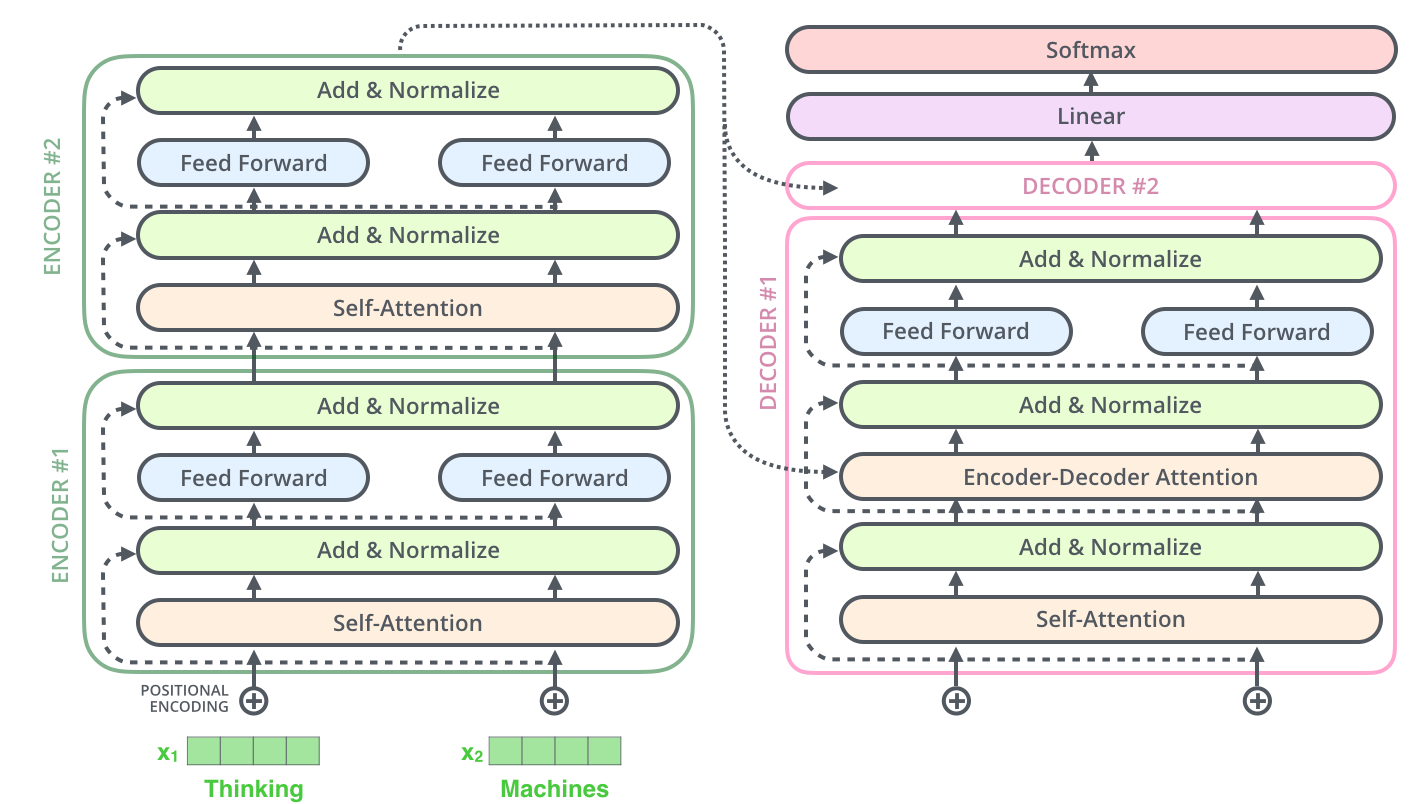
\includegraphics[width=0.8\textwidth]{imgs/encoderDecoderLayersDetailed.png}
\vspace{-10pt}
\caption{\footnotesize The layers inside Encoder and Decoder. From \emph{The Illustrated Transformer}, by Alammar, 2018. \url{https://jalammar.github.io/illustrated-transformer/}. Copyright 2018 by Alammar.}
\vspace{-5pt}
\label{fig:encDecLayersDetailed}
\end{figure}




\subsection{Decoder} \label{sec:TransformerDecoder}


The Decoder \hyperref[sec:NeuralLM]{neural network} generates hidden states $s_t = \text{Decoder}\Big( s_{t-1}, y_{t-1}, c_t \Big)$ for time steps $t = 1,..., m$ where the context vector $c_t = \sum_{i=1}^n \alpha_{ti} \cdot h_i$ is a sum of the hidden states of the input sentence, weighted by alignment scores, as for the \hyperref[sec:Seq2Seq]{Seq-to-Seq} model (Weng, 2018). 

Similarly to the Encoder, the Decoder contains a stack of $N$ Decoder layers, each of which consist of several sub-layers:
\begin{enumerate}
    \item \textbf{ \nameref{sec:MaskedMultiHeadAttention} (layer)}
    \item \textbf{ \nameref{sec:EncoderDecoderAttention} (layer)} 
    \item \textbf{ \nameref{sec:PositionwiseFFNLayers} (layer) }. 
\end{enumerate}

Like in the Encoder, in between each of these layers is a \hyperref[sec:ResidualConnections]{residual connection} followed by layer normalization. The Encoder and Decoder stack are shown in \cref{fig:encDecLayersDetailed}. 




\subsection{Final Linear and Softmax Layer} \label{sec:TransformerFinalLayer}


The Decoder stack outputs a vector of floats which is converted to a word using a Linear layer, followed by a Softmax layer in the Transformer neural network (Alammar, 2018b). 
\begin{itemize}
    \item \textbf{Linear Layer} is a simple, \hyperref[sec:NeuralLM]{fully-connected neural network} that projects the Decoder's output vector in a larger-dimension ``logits vector" in which each cell holds a score corresponding to each unique vocabulary word. 
    
    \item \textbf{Softmax Layer} then converts the Linear Layer's scores into probabilities via the \hyperref[cnc:softmaxLayer]{softmax function}. 
\end{itemize}

To find the predicted word, the cell with highest probability is chosen, and corresponding word is called the predicted word, and is output for a particular time step.




\subsection{Transformer Workflow} \label{sec:TransformerWorkflow}

Alammar (2018b) describes the procedure governing the Transformer's moving parts as follows: 

\begin{enumerate}
    \item The \nameref{sec:TransformerEncoder} processes the input sentence in the given language, adding the \hyperref[sec:PosEncodings]{positional encoding} to input embeddings.
    
    \item The output of the top \nameref{sec:TransformerEncoder} layer is then transformed into a set of \hyperref[sec:AttentionMechanism]{attention} vectors $K$ and $V$.
    
    \item The \nameref{sec:TransformerDecoder} uses $K$ and $V$ in its \hyperref[sec:EncoderDecoderAttention]{encoder-decoder attention layer} to help the \nameref{sec:TransformerDecoder} focus on appropriate places in the input sequence. Subsequent outputs are fed to the bottom \nameref{sec:TransformerDecoder}, allowing \nameref{sec:TransformerDecoder}s to accumulate results. Also, the \nameref{sec:TransformerDecoder} includes \hyperref[sec:PosEncodings]{positional encoding}s to its inputs. 
    
    \item The previous steps are repeated until a special symbol is reached, indicated the \nameref{sec:TransformerDecoder} has finished generating output.
    
    \item The \nameref{sec:TransformerDecoder}'s numeric output vector is passed through the \hyperref[sec:TransformerFinalLayer]{final linear and softmax layer} to find a predicted, translated word in the target language. 
    
\end{enumerate}

